% ============================================================
% BidKV: Quality-Aware Preemption Scheduling
%        for KV-Pressure LLM Serving
% SC 2026 — ACM sigconf format
% ============================================================
\documentclass[sigconf,nonacm]{acmart}

% ------------------------------------------------------------
% Packages
% ------------------------------------------------------------
\usepackage{amsmath}
% amssymb loaded before newtxmath to avoid \Bbbk clash
\let\Bbbk\undefined
\usepackage{amssymb}
\usepackage{booktabs}
\usepackage{algorithm}
\usepackage{algpseudocode}
\usepackage{tikz}
\usetikzlibrary{arrows.meta, decorations.pathreplacing, positioning, calc}
\usepackage{subcaption}
\usepackage{xcolor}
\usepackage{xspace}
\usepackage{multirow}
\usepackage{enumitem}
\usepackage{balance}
\usepackage{pifont}  % \ding symbols for circled numbers in figures
\usepackage{graphicx}

% Allow slightly looser line breaking to prevent overfull hboxes
\emergencystretch=1.5em

% ------------------------------------------------------------
% Placeholder command — experimental data filled after Wave 4
% ------------------------------------------------------------
\newcommand{\placeholder}[1]{\textcolor{red}{\textbf{#1}}}

% Named data macros — v8 mixed-workload frozen data

% Shorthand
\newcommand{\bidkv}{BidKV\xspace}
\newcommand{\sys}{\bidkv}
\newcommand{\utilfn}{\ensuremath{U}}
\newcommand{\tokfree}{\ensuremath{r}}
\newcommand{\qualdelta}{\ensuremath{\delta}}
\newcommand{\stabeps}{\ensuremath{\varepsilon}}
\newcommand{\dbudget}{\ensuremath{\Delta_{\max}}}
\newcommand{\neededtok}{\ensuremath{N}}
\newcommand{\numbids}{\ensuremath{B}}

% Citation shortcuts
\newcommand{\eg}{\emph{e.g.},\xspace}
\newcommand{\ie}{\emph{i.e.},\xspace}
\newcommand{\etc}{\emph{etc.}\xspace}
\newcommand{\etal}{\emph{et al.}\xspace}

% ============================================================
\begin{document}

% ------------------------------------------------------------
% Title & Authors
% ------------------------------------------------------------
\title{BidKV: Utility-Guided Preemption Scheduling for KV-Pressure LLM Serving}

\author{Anonymous Authors}
\affiliation{%
  \institution{Anonymous Institution}
  \country{}
}

% ============================================================
% Abstract
% ============================================================
\begin{abstract}
When KV-cache demand exceeds GPU memory capacity during online LLM serving, serving engines reclaim cache from active requests to admit waiting ones. Poor victim selection wastes recomputation, delays admission of queued requests, and degrades first-token latency---a metric directly visible to users. Existing policies rely on coarse request-order heuristics (LIFO, FCFS) or independent per-request scoring rules, lacking both explicit reclamation-cost signals and cross-request coordination. We present BidKV, a utility-guided reclamation policy that improves \emph{admission responsiveness} under KV pressure. Each active request produces a bid encoding recoverable capacity and estimated disruption cost; a coordinated solver selects victims that free the required capacity at minimum aggregate cost. The current prototype instantiates disruption cost from request-lifecycle proxies (completion progress, prompt length, preemption history) under recompute-fallback semantics. BidKV integrates non-invasively with vLLM and SGLang via a portable adapter layer. Evaluated with Llama-3.1-8B-Instruct on an NVIDIA RTX A6000 under ShareGPT traces, BidKV reduces P95 TTFT by 89\% and improves 300\,ms SLO attainment by 14.9\,pp over vLLM's native policy, at comparable throughput.
\end{abstract}

\maketitle

% ============================================================
% §1  Introduction
% ============================================================
\section{Introduction}\label{sec:intro}

Online large language model~(LLM) serving must sustain a continuously changing
population of concurrent requests on limited GPU memory.  In production
workloads, requests are highly heterogeneous in prompt length, generation
budget, and arrival pattern; they also progress asynchronously as some requests
are still in prefill while others are already deep into
decoding~\cite{Kwon2023, Yu2022, Zheng2024lmsys}.  Under such mixed-length,
bursty workloads, the key-value~(KV) cache becomes a dominant runtime
resource~\cite{Vaswani2017, Pope2022}: new arrivals
allocate KV state, ongoing requests expand it token by token, and completed or
preempted requests release it at different points in their lifecycle.  Aggregate
KV demand therefore fluctuates on short timescales and can repeatedly exceed
available capacity during normal operation, forcing the serving engine to
reclaim KV state from active requests to make room for others.

The central question in this setting is not whether KV capacity must be
reclaimed, but which active request should be chosen as the \emph{victim}.
Two requests may occupy comparable amounts of KV memory while imposing very
different costs when interrupted.  Under the \emph{recompute-fallback}
execution model used by current serving engines~\cite{Kwon2023}, reclaiming an
active request releases its KV state but forces the request to restart through
the framework's native recovery path when it is rescheduled.  The cost of reclamation therefore
depends not only on how much memory is freed, but also on how much useful
computation is discarded and must later be redone.  Reclaiming a request that is
near completion can waste substantial prior work and incur expensive
recomputation, whereas reclaiming a request that has only recently entered
decoding may free similar capacity at much lower system disruption.  Poor victim
choices can also cascade: recomputation re-inflates KV demand, which in turn
triggers further reclamation---a cycle that keeps KV capacity occupied by
recomputing victims rather than available for waiting requests.  The direct
consequence is admission-latency degradation: queued requests wait longer to
receive their first token, driving up time-to-first-token~(TTFT) and eroding
service-level objective~(SLO) attainment.  Active-KV reclamation is therefore a
cross-request victim-selection problem whose quality directly governs admission
responsiveness under sustained KV pressure.

Because reclamation costs are heterogeneous, the scheduler needs
\emph{explicit per-request cost signals} to distinguish cheap victims from
expensive ones; because selection is cross-request, these signals must feed
into \emph{coordinated batch-level selection} rather than independent
per-request rules.  No existing system provides both.  Current scheduling
heuristics---LIFO preemption~\cite{Kwon2023}, FCFS
admission~\cite{Yu2022}, EDF-style waiting
policies~\cite{Gujarati2020}---determine victim order without any
per-request cost signal; broader serving innovations such as chunked
prefills~\cite{Agrawal2024sarathiserve} and prefill--decode
disaggregation~\cite{Zhong2024, Patel2024} advance throughput and resource
placement but inherit the same order-based victim selection, leaving the
signal gap intact.  Token-level scoring methods such as
H2O~\cite{Zhang2023h2o} and StreamingLLM~\cite{Xiao2024} do produce
request-specific importance signals, yet each applies a fixed scoring rule
independently---without coordination across the batch, a locally reasonable
per-request choice can be globally costly.  What is missing is a
\emph{signal pathway}: a structured interface through which per-request
reclamation sensitivity can be surfaced to the scheduler and used for
coordinated cross-request victim selection.

In this study we present \bidkv, a \emph{bid-based scheduling abstraction} for
active-KV reclamation.  The key idea is to make reclamation sensitivity an
explicit, structured signal rather than an implicit consequence of scheduling
order.  Each active request produces a \emph{bid} that summarizes the KV
capacity recoverable upon reclamation and a surrogate disruption estimate
reflecting the relative penalty of reclaiming that request.  Given bids from all
active requests, the scheduler solves a constrained cross-request selection
problem: choose the victim set that recovers the required capacity while
minimizing aggregate estimated disruption.  In this way, \bidkv turns victim
selection from an opaque runtime behavior into an explicit interface between a
\emph{scoring layer}---which estimates per-request reclamation
sensitivity---and a \emph{coordinated selection layer}---which makes
batch-level trade-offs across candidates.

In the current prototype, the disruption estimate is instantiated from
request-lifecycle features (completion progress, prompt length, preemption
history) under recompute-fallback semantics~\cite{Kwon2023}.
\bidkv integrates non-invasively with both vLLM~\cite{Kwon2023} and
SGLang~\cite{Zheng2024sglang} via a portable adapter layer that fully reuses
each framework's native reclamation and recovery paths---the fact that both
integrations require no source-code modification confirms that the bid
interface is cleanly separated from framework-specific scheduling internals.
\bidkv controls \emph{which} request is reclaimed, not \emph{how}.  Under
recompute-fallback execution, the policy does not alter final outputs; the
differentiation lies entirely in scheduling efficiency.  The primary benefit is
improved admission responsiveness: by selecting victims whose reclamation
frees adequate capacity at low recompute cost, \bidkv reduces the time
waiting requests spend queued for KV allocation, yielding lower TTFT and
higher SLO attainment.  This comes at a modest cost in throughput and
per-token decode latency, a tradeoff that favors latency-sensitive
deployments.  The benefit is operating-regime dependent: under sustained
mixed-length KV pressure, utility-guided selection provides substantial
gains; under low pressure, victim selection remains governed by the
framework's native ordering, with \bidkv's reorder activating only under
sustained high-pressure conditions.

\paragraph{Contributions.}
\begin{enumerate}[leftmargin=*,nosep]
\item \textbf{Bid-based reclamation interface.}
  We introduce a structured bid abstraction that allows per-request
  reclamation sensitivity to be surfaced to the runtime scheduler, replacing
  implicit victim ordering rules with an explicit decision interface.

\item \textbf{Decoupled scoring-to-selection architecture.}
  We separate request-level disruption estimation from coordinated
  cross-request victim selection through a structured bid interface,
  so that selection operates on uniform cost--capacity pairs regardless
  of how disruption estimates are produced.

\item \textbf{Portable runtime integration.}
  We realize \bidkv as a non-invasive scheduling layer with a
  \texttt{Framework\-Adapter} abstraction, demonstrating integration with
  vLLM and SGLang that reuses each framework's native reclamation and
  recovery mechanisms without source-code modification.

\item \textbf{Structured evaluation under controlled conditions.}
  We evaluate five strategies that vary across scheduling dimensions
  (admission ordering, running-queue reordering, victim selection logic,
  and proactive reclamation) under frozen request traces and calibrated
  arrival rates, supporting structured attribution across these co-varying
  dimensions.
\end{enumerate}

% ============================================================
% §2  Background and Motivation
% ============================================================
\section{Background and Motivation}\label{sec:background}

\subsection{KV Cache Memory Model}\label{sec:bg:kvcache}

Each autoregressive decoding step caches key and value
projections~\cite{Vaswani2017} for all previously generated tokens.  For a
model with $L$~layers, $H$~KV heads (via grouped-query
attention~\cite{Ainslie2023}), and head dimension~$d_h$, a single request of
length~$n$ stores $2LHd_h n$ elements.  With bf16 precision, Llama-3.1-8B-Instruct ($L{=}32,
H{=}8_{\text{kv}}, d_h{=}128$) allocates 128\,KiB per token per
request~\cite{Grattafiori2024}.  vLLM~\cite{Kwon2023} manages this state through
PagedAttention: physical GPU memory is partitioned into fixed-size \emph{blocks}
that are mapped to logical positions via a block table.  On a 48\,GiB
A6000 with $\sim$16\,GiB occupied by model weights~\cite{Pope2023}, the
remaining $\sim$32\,GiB of KV-allocatable memory can sustain roughly 260K
tokens of concurrent KV state---a single 4096-token request already consumes
$\sim$512\,MiB, or about 1.6\% of total KV capacity.

\subsection{The Victim-Selection Problem}\label{sec:bg:preemption}

When aggregate KV demand exceeds available capacity, the serving engine must
reclaim KV state from one or more active requests.  Under recompute-fallback
semantics~\cite{Kwon2023}, the victim's KV blocks are released and the request
re-enters the waiting queue; when it is eventually rescheduled, its prompt is
recomputed from scratch.  The scheduler's task at each reclamation event is
therefore to choose a \emph{victim set} $V \subseteq \mathcal{R}$ from the set
of active requests~$\mathcal{R}$ such that the total freed capacity meets the
shortfall while minimizing aggregate recompute cost:

\begin{equation}\label{eq:victim}
  \min_{V \subseteq \mathcal{R}} \sum_{i \in V} c_i
  \quad \text{s.t.} \quad
  \sum_{i \in V} r_i \;\geq\; N,
\end{equation}

\noindent
where $r_i$ is the KV capacity freed by reclaiming request~$i$, $c_i$ is the
recompute cost it will incur, and $N$ is the capacity shortfall.  This
formulation is an instance of the minimum-cost covering
problem~\cite{Kellerer2004}.  With
heterogeneous requests, the choice of~$V$ matters: two requests may free
comparable capacity yet differ by an order of magnitude in recompute cost.
Existing engines do not solve this selection problem explicitly.  vLLM selects
the most recently scheduled request (LIFO)~\cite{Kwon2023}; other systems apply
FCFS~\cite{Yu2022} or EDF ordering~\cite{Gujarati2020}, none of which accounts
for per-request reclamation cost.  This
analysis motivates two requirements.  First, the scheduler should accept
\emph{explicit per-request reclamation-sensitivity signals} that capture
heterogeneity in reclamation cost, rather than relying solely on arrival or
scheduling order.  Second, victim selection should perform \emph{cross-request
coordination}---considering the batch-level trade-off between KV capacity freed
and recompute cost incurred---rather than scoring each request in isolation.


\paragraph{Empirical evidence.}
Figure~\ref{fig:motivation} validates the above analysis with a KV-pressure
snapshot drawn from a long-context ShareGPT trace (rate=0.5\,req/s).  We use a
long-context scenario for this illustration because it amplifies per-request KV
heterogeneity, making the victim-selection gap between LIFO and utility-guided
policies maximally visible; the same gap arises under mixed-length workloads
(Section~\ref{sec:eval}) at smaller absolute scale.
Panel~(a) shows 10 concurrent requests at the moment of peak KV utilization,
sorted by tokens held.
LIFO targets R1 and R2---the requests with the largest KV footprints---yet
these requests are 47\% and 34\% complete, incurring estimated recompute costs
of $\sim$1{,}800 and $\sim$1{,}050~tokens respectively (red hatched bars).
A utility-guided policy instead selects~R4, which is only~3\% complete: it
frees 1{,}825~tokens while imposing a recompute cost of just~62~tokens---a
29$\times$ improvement in recompute efficiency for this single victim choice.

Panel~(b) aggregates the comparison over a target of freeing 20\% of total KV
capacity.
LIFO recovers 1.4$\times$ more tokens per event (by preferring larger
requests), but at a 5.0$\times$ higher average recompute cost and a
1.2$\times$ larger estimated cascade factor---the multiplier reflecting
re-inflation of KV pressure as recomputed requests re-enter the running queue
and re-acquire KV blocks.
Coarse victim selection trades marginal extra KV recovery for a
disproportionate recompute burden, compounding tail-latency degradation at
every subsequent scheduling step.

\begin{figure}[t]
\centering
\includegraphics[width=\columnwidth]{figures/fig_preliminary_motivation.pdf}
\caption{Empirical motivation (long-context trace, ShareGPT, rate=0.5\,req/s).
  \textbf{(a)}~Per-request KV footprint (blue) and estimated recompute cost
  (red hatched) at a KV-pressure snapshot; 10 concurrent requests sorted by
  KV tokens held, high$\to$low.
  LIFO targets R1--R2 (34--47\% complete); utility-guided selects R4
  (3\% complete, $29\times$ lower recompute cost).
  \textbf{(b)}~Aggregate comparison freeing 20\% of total KV capacity:
  LIFO imposes 5.0$\times$ higher average recompute cost and 1.2$\times$
  larger cascade factor relative to utility-guided selection.}
\label{fig:motivation}
\end{figure}


% ============================================================
% §3  Related Work
% ============================================================
\section{Related Work}\label{sec:related}

\paragraph{Request-level scheduling and preemption.}
vLLM~\cite{Kwon2023} introduced PagedAttention with request-level preemption
(swap or recompute) as the fallback under memory pressure.
Orca~\cite{Yu2022} pioneered iteration-level scheduling but does not manage KV
capacity.
DistServe~\cite{Zhong2024} and Splitwise~\cite{Patel2024} disaggregate prefill
and decode phases, while
Sarathi-Serve~\cite{Agrawal2024sarathiserve} introduces chunked prefills.
FlexGen~\cite{Sheng2023flexgen} offloads KV cache to CPU/disk.
LoongServe~\cite{Wu2024loongserve} scales to long contexts via elastic
partitioning.
Prompt Cache~\cite{Gim2024} and Hydragen~\cite{Juravsky2024} exploit prefix
sharing to reduce redundant computation.
These systems advance batching, placement, and memory management, but their
preemption policies remain order-based (LIFO or FCFS) and do not incorporate
per-request cost signals when selecting victims.

\paragraph{Token-level KV cache compression.}
H2O~\cite{Zhang2023h2o} identifies ``heavy-hitter'' tokens via
cumulative attention scores.
Streaming\-LLM~\cite{Xiao2024} preserves attention-sink tokens
for infinite streaming.
Scissorhands~\cite{Liu2023scissorhands} exploits persistence-of-importance.
SnapKV~\cite{Li2024snapkv} clusters attention features to compress prefix
cache.
KIVI~\cite{Liu2024kivi} uses asymmetric 2-bit KV quantization.
PyramidKV~\cite{Zhang2025pyramidkv} applies pyramid budgets across layers.
These methods effectively reduce per-request KV footprint, but each applies a
fixed budget and scoring rule to every request independently.  They do not
coordinate across the batch to reason about which \emph{request} to target, nor
do they expose a hook for external policies to influence the decision.
\bidkv is complementary: its scoring layer can wrap any token-level scorer (\eg
H2O) to derive per-request bid signals for cross-request coordination.

\paragraph{System-level QoS and scheduling theory.}
Dominant Resource Fairness~\cite{Ghodsi2011} and multi-resource
packing~\cite{Grandl2014} optimize heterogeneous cluster resources.
The knapsack literature~\cite{Martello1990, Kellerer2004} provides algorithmic
foundations for constrained selection.
These frameworks operate on compute or network resources, not KV cache capacity,
and do not incorporate the per-request preemption-sensitivity signals that arise
in LLM serving.

\paragraph{Positioning.}
To our knowledge, no prior work provides an explicit, scorer-agnostic signal
pathway through which per-request preemption sensitivity can be communicated to
the KV cache scheduler and used for cross-request victim coordination.
\bidkv aims to fill this gap: it is complementary to token-level compression
methods (which supply scoring signals) and to request-level scheduling systems
(which supply the preemption execution mechanism).

% ============================================================
% §4  Design
% ============================================================
\section{Design}\label{sec:design}

The victim-selection problem identified in Section~\ref{sec:background}
imposes two requirements: explicit reclamation-sensitivity signals and
cross-request coordination.  Two additional design goals guide our architecture:
\emph{scorer-agnostic interface}---because the best importance signal may vary
across workloads and models, the scoring strategy should be interchangeable
without modifying the selection algorithm or the runtime integration; and
\emph{framework portability}---the mechanism should integrate with heterogeneous
serving engines (\eg vLLM, SGLang) by reusing their native reclamation and
recovery paths, without requiring source-code modifications.

These goals separate naturally into a \emph{general architecture}---the
bid-based data path and layered decomposition that are execution-model
agnostic---and a \emph{current instantiated path}---the specific disruption
estimator ($\qualdelta$, Eq.~\ref{eq:delta}) that uses request-lifecycle
features under recompute-fallback semantics.  The architecture prescribes how
scoring signals flow to the solver; the instantiation determines which features
populate $\qualdelta$ in this paper.

\noindent
\bidkv organizes its logic into four layers (Figure~\ref{fig:architecture}): the
\emph{Runtime Adapter Layer} detects KV pressure and executes reclamations via
the framework's native mechanism; the \emph{Scoring-to-Bid Layer} translates
token-level scores into structured bids; the \emph{Constrained Solver Layer}
selects reclamation victims; and the \emph{Bid Signal Layer} defines the shared
data structures used across all layers.

% fig1_architecture.tex — BidKV Four-Layer Architecture (TikZ)
% Usage: % fig1_architecture.tex — BidKV Four-Layer Architecture (TikZ)
% Usage: % fig1_architecture.tex — BidKV Four-Layer Architecture (TikZ)
% Usage: \input{figures/fig1_architecture}
%
% Layout: four layers stacked bottom-to-top by abstraction level.
% Left arrows (blue, upward)  = invocation / trigger flow
% Right arrows (orange, downward) = data / result flow
% Updated for preemption scheduling narrative (v2)

\begin{figure}[t]
\centering
\resizebox{\columnwidth}{!}{%
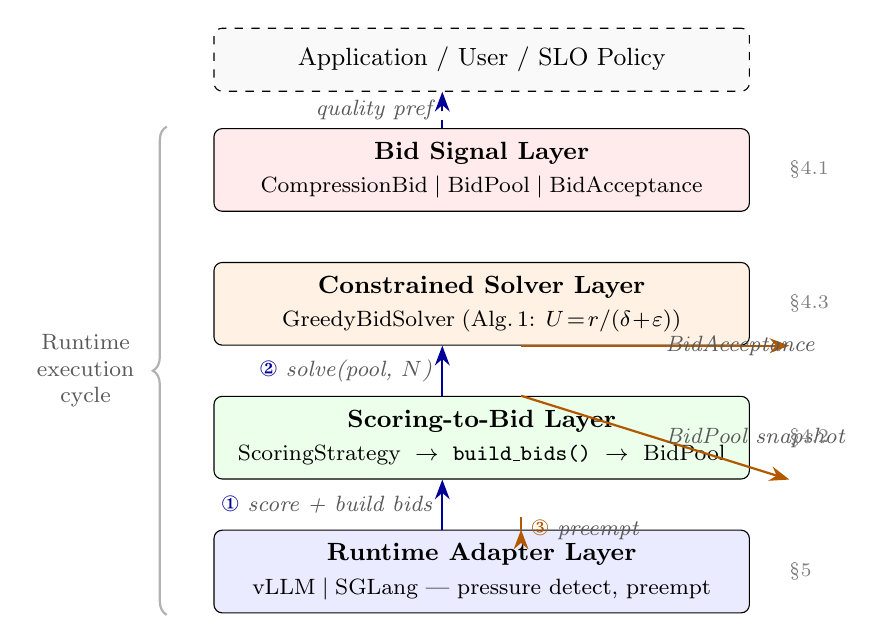
\begin{tikzpicture}[
  layer/.style={draw, rounded corners=3pt, minimum width=6.8cm, minimum height=1.05cm,
                align=center, font=\small},
  callarrow/.style={-{Stealth[length=2.5mm]}, thick, blue!60!black},
  dataarrow/.style={-{Stealth[length=2.5mm]}, thick, orange!70!black},
  lbl/.style={font=\footnotesize\itshape, text=gray!70!black},
]

% ---- Layers (bottom = runtime, top = protocol) ----

% Layer 4 — Runtime Adapter (bottom)
\node[layer, fill=blue!8] (L4) at (0, 0)
  {\textbf{Runtime Adapter Layer}\\[1pt]
   {\footnotesize vLLM\;\textbar\;SGLang — pressure detect, preempt}};

% Layer 3 — Scoring-to-Bid
\node[layer, fill=green!8] (L3) at (0, 1.7)
  {\textbf{Scoring-to-Bid Layer}\\[1pt]
   {\footnotesize ScoringStrategy $\;\to\;$ \texttt{build\_bids()} $\;\to\;$ BidPool}};

% Layer 2 — Constrained Solver
\node[layer, fill=orange!10] (L2) at (0, 3.4)
  {\textbf{Constrained Solver Layer}\\[1pt]
   {\footnotesize GreedyBidSolver\;(Alg.\,1: $U\!=\!r/(\delta\!+\!\varepsilon)$)}};

% Layer 1 — Bid Signal (protocol definitions)
\node[layer, fill=red!8] (L1) at (0, 5.1)
  {\textbf{Bid Signal Layer}\\[1pt]
   {\footnotesize CompressionBid\;\textbar\;BidPool\;\textbar\;BidAcceptance}};

% External — Application / User
\node[draw, dashed, rounded corners=3pt, minimum width=6.8cm, minimum height=0.8cm,
      align=center, font=\small, fill=gray!5] (App) at (0, 6.5)
  {Application / User / SLO Policy};

% ---- Left side: invocation flow (blue, upward) ----
\draw[callarrow] ([xshift=-5mm]L4.north) -- ([xshift=-5mm]L3.south)
  node[midway, left, lbl] {\textcolor{blue!60!black}{\ding{172}} score + build bids};
\draw[callarrow] ([xshift=-5mm]L3.north) -- ([xshift=-5mm]L2.south)
  node[midway, left, lbl] {\textcolor{blue!60!black}{\ding{173}} solve(pool, $N$)};
\draw[callarrow, dashed] ([xshift=-5mm]L1.north) -- ([xshift=-5mm]App.south)
  node[midway, left, lbl] {quality pref};

% ---- Right side: data / result flow (orange, downward) ----
\draw[dataarrow] ([xshift=5mm]L3.north) -- ([xshift=5mm]L4.north east |- L3.south)
  node[midway, right, lbl] {BidPool snapshot};
\draw[dataarrow] ([xshift=5mm]L2.south) -- ([xshift=5mm]L3.north east |- L2.south)
  node[midway, right, lbl] {BidAcceptance};
\draw[dataarrow] ([xshift=5mm]L2.south |- L4.north) -- ([xshift=5mm]L4.north)
  node[midway, right, lbl] {\textcolor{orange!70!black}{\ding{174}} preempt};

% ---- Section annotations (far right) ----
\node[font=\scriptsize, text=gray, anchor=west] at (3.8, 0)    {\S5};
\node[font=\scriptsize, text=gray, anchor=west] at (3.8, 1.7)  {\S4.2};
\node[font=\scriptsize, text=gray, anchor=west] at (3.8, 3.4)  {\S4.3};
\node[font=\scriptsize, text=gray, anchor=west] at (3.8, 5.1)  {\S4.1};

% ---- Left brace ----
\draw[decorate, decoration={brace, amplitude=5pt}, thick, gray!60]
  (-4.0, -0.55) -- (-4.0, 5.65)
  node[midway, left=8pt, font=\footnotesize, text=gray!70!black, align=center]
  {Runtime\\execution\\cycle};

\end{tikzpicture}%
}% end resizebox
\caption{BidKV four-layer architecture.  Upon KV pressure, the
adapter~(\ding{172}) invokes the scoring layer to generate bids,
(\ding{173})~passes the bid pool to the solver, and
(\ding{174})~executes the returned acceptance via the framework's
native preemption API.  Blue (left) arrows show the invocation flow;
orange (right) arrows show the data/result flow.  The bid signal
layer (top) defines the protocol data structures shared across all
layers.}
\label{fig:architecture}
\end{figure}

%
% Layout: four layers stacked bottom-to-top by abstraction level.
% Left arrows (blue, upward)  = invocation / trigger flow
% Right arrows (orange, downward) = data / result flow
% Updated for preemption scheduling narrative (v2)

\begin{figure}[t]
\centering
\resizebox{\columnwidth}{!}{%
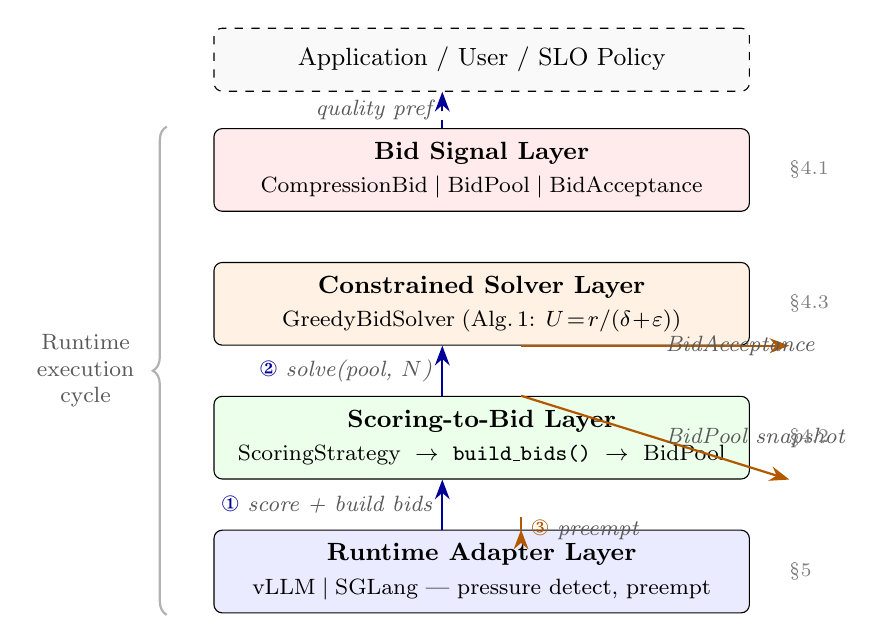
\begin{tikzpicture}[
  layer/.style={draw, rounded corners=3pt, minimum width=6.8cm, minimum height=1.05cm,
                align=center, font=\small},
  callarrow/.style={-{Stealth[length=2.5mm]}, thick, blue!60!black},
  dataarrow/.style={-{Stealth[length=2.5mm]}, thick, orange!70!black},
  lbl/.style={font=\footnotesize\itshape, text=gray!70!black},
]

% ---- Layers (bottom = runtime, top = protocol) ----

% Layer 4 — Runtime Adapter (bottom)
\node[layer, fill=blue!8] (L4) at (0, 0)
  {\textbf{Runtime Adapter Layer}\\[1pt]
   {\footnotesize vLLM\;\textbar\;SGLang — pressure detect, preempt}};

% Layer 3 — Scoring-to-Bid
\node[layer, fill=green!8] (L3) at (0, 1.7)
  {\textbf{Scoring-to-Bid Layer}\\[1pt]
   {\footnotesize ScoringStrategy $\;\to\;$ \texttt{build\_bids()} $\;\to\;$ BidPool}};

% Layer 2 — Constrained Solver
\node[layer, fill=orange!10] (L2) at (0, 3.4)
  {\textbf{Constrained Solver Layer}\\[1pt]
   {\footnotesize GreedyBidSolver\;(Alg.\,1: $U\!=\!r/(\delta\!+\!\varepsilon)$)}};

% Layer 1 — Bid Signal (protocol definitions)
\node[layer, fill=red!8] (L1) at (0, 5.1)
  {\textbf{Bid Signal Layer}\\[1pt]
   {\footnotesize CompressionBid\;\textbar\;BidPool\;\textbar\;BidAcceptance}};

% External — Application / User
\node[draw, dashed, rounded corners=3pt, minimum width=6.8cm, minimum height=0.8cm,
      align=center, font=\small, fill=gray!5] (App) at (0, 6.5)
  {Application / User / SLO Policy};

% ---- Left side: invocation flow (blue, upward) ----
\draw[callarrow] ([xshift=-5mm]L4.north) -- ([xshift=-5mm]L3.south)
  node[midway, left, lbl] {\textcolor{blue!60!black}{\ding{172}} score + build bids};
\draw[callarrow] ([xshift=-5mm]L3.north) -- ([xshift=-5mm]L2.south)
  node[midway, left, lbl] {\textcolor{blue!60!black}{\ding{173}} solve(pool, $N$)};
\draw[callarrow, dashed] ([xshift=-5mm]L1.north) -- ([xshift=-5mm]App.south)
  node[midway, left, lbl] {quality pref};

% ---- Right side: data / result flow (orange, downward) ----
\draw[dataarrow] ([xshift=5mm]L3.north) -- ([xshift=5mm]L4.north east |- L3.south)
  node[midway, right, lbl] {BidPool snapshot};
\draw[dataarrow] ([xshift=5mm]L2.south) -- ([xshift=5mm]L3.north east |- L2.south)
  node[midway, right, lbl] {BidAcceptance};
\draw[dataarrow] ([xshift=5mm]L2.south |- L4.north) -- ([xshift=5mm]L4.north)
  node[midway, right, lbl] {\textcolor{orange!70!black}{\ding{174}} preempt};

% ---- Section annotations (far right) ----
\node[font=\scriptsize, text=gray, anchor=west] at (3.8, 0)    {\S5};
\node[font=\scriptsize, text=gray, anchor=west] at (3.8, 1.7)  {\S4.2};
\node[font=\scriptsize, text=gray, anchor=west] at (3.8, 3.4)  {\S4.3};
\node[font=\scriptsize, text=gray, anchor=west] at (3.8, 5.1)  {\S4.1};

% ---- Left brace ----
\draw[decorate, decoration={brace, amplitude=5pt}, thick, gray!60]
  (-4.0, -0.55) -- (-4.0, 5.65)
  node[midway, left=8pt, font=\footnotesize, text=gray!70!black, align=center]
  {Runtime\\execution\\cycle};

\end{tikzpicture}%
}% end resizebox
\caption{BidKV four-layer architecture.  Upon KV pressure, the
adapter~(\ding{172}) invokes the scoring layer to generate bids,
(\ding{173})~passes the bid pool to the solver, and
(\ding{174})~executes the returned acceptance via the framework's
native preemption API.  Blue (left) arrows show the invocation flow;
orange (right) arrows show the data/result flow.  The bid signal
layer (top) defines the protocol data structures shared across all
layers.}
\label{fig:architecture}
\end{figure}

%
% Layout: four layers stacked bottom-to-top by abstraction level.
% Left arrows (blue, upward)  = invocation / trigger flow
% Right arrows (orange, downward) = data / result flow
% Updated for preemption scheduling narrative (v2)

\begin{figure}[t]
\centering
\resizebox{\columnwidth}{!}{%
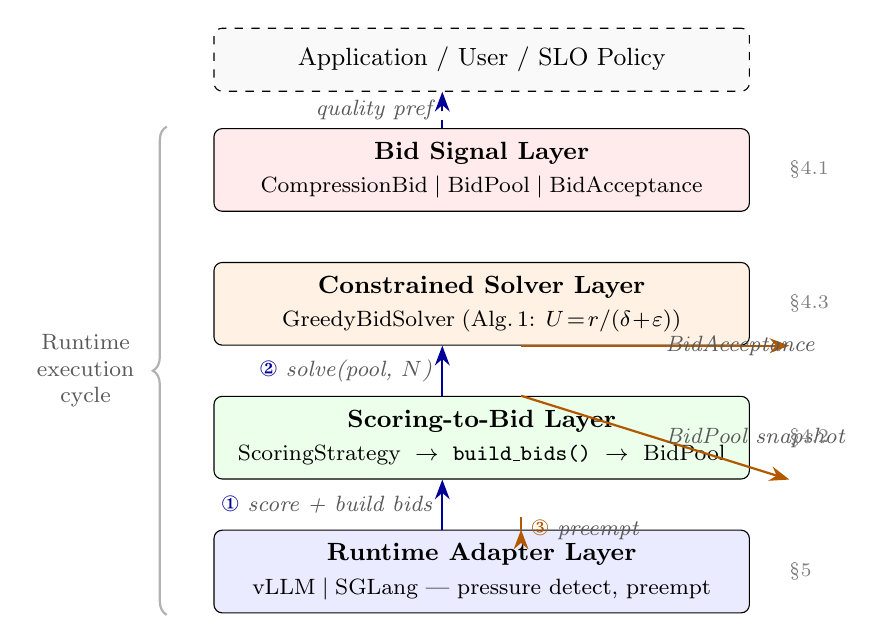
\begin{tikzpicture}[
  layer/.style={draw, rounded corners=3pt, minimum width=6.8cm, minimum height=1.05cm,
                align=center, font=\small},
  callarrow/.style={-{Stealth[length=2.5mm]}, thick, blue!60!black},
  dataarrow/.style={-{Stealth[length=2.5mm]}, thick, orange!70!black},
  lbl/.style={font=\footnotesize\itshape, text=gray!70!black},
]

% ---- Layers (bottom = runtime, top = protocol) ----

% Layer 4 — Runtime Adapter (bottom)
\node[layer, fill=blue!8] (L4) at (0, 0)
  {\textbf{Runtime Adapter Layer}\\[1pt]
   {\footnotesize vLLM\;\textbar\;SGLang — pressure detect, preempt}};

% Layer 3 — Scoring-to-Bid
\node[layer, fill=green!8] (L3) at (0, 1.7)
  {\textbf{Scoring-to-Bid Layer}\\[1pt]
   {\footnotesize ScoringStrategy $\;\to\;$ \texttt{build\_bids()} $\;\to\;$ BidPool}};

% Layer 2 — Constrained Solver
\node[layer, fill=orange!10] (L2) at (0, 3.4)
  {\textbf{Constrained Solver Layer}\\[1pt]
   {\footnotesize GreedyBidSolver\;(Alg.\,1: $U\!=\!r/(\delta\!+\!\varepsilon)$)}};

% Layer 1 — Bid Signal (protocol definitions)
\node[layer, fill=red!8] (L1) at (0, 5.1)
  {\textbf{Bid Signal Layer}\\[1pt]
   {\footnotesize CompressionBid\;\textbar\;BidPool\;\textbar\;BidAcceptance}};

% External — Application / User
\node[draw, dashed, rounded corners=3pt, minimum width=6.8cm, minimum height=0.8cm,
      align=center, font=\small, fill=gray!5] (App) at (0, 6.5)
  {Application / User / SLO Policy};

% ---- Left side: invocation flow (blue, upward) ----
\draw[callarrow] ([xshift=-5mm]L4.north) -- ([xshift=-5mm]L3.south)
  node[midway, left, lbl] {\textcolor{blue!60!black}{\ding{172}} score + build bids};
\draw[callarrow] ([xshift=-5mm]L3.north) -- ([xshift=-5mm]L2.south)
  node[midway, left, lbl] {\textcolor{blue!60!black}{\ding{173}} solve(pool, $N$)};
\draw[callarrow, dashed] ([xshift=-5mm]L1.north) -- ([xshift=-5mm]App.south)
  node[midway, left, lbl] {quality pref};

% ---- Right side: data / result flow (orange, downward) ----
\draw[dataarrow] ([xshift=5mm]L3.north) -- ([xshift=5mm]L4.north east |- L3.south)
  node[midway, right, lbl] {BidPool snapshot};
\draw[dataarrow] ([xshift=5mm]L2.south) -- ([xshift=5mm]L3.north east |- L2.south)
  node[midway, right, lbl] {BidAcceptance};
\draw[dataarrow] ([xshift=5mm]L2.south |- L4.north) -- ([xshift=5mm]L4.north)
  node[midway, right, lbl] {\textcolor{orange!70!black}{\ding{174}} preempt};

% ---- Section annotations (far right) ----
\node[font=\scriptsize, text=gray, anchor=west] at (3.8, 0)    {\S5};
\node[font=\scriptsize, text=gray, anchor=west] at (3.8, 1.7)  {\S4.2};
\node[font=\scriptsize, text=gray, anchor=west] at (3.8, 3.4)  {\S4.3};
\node[font=\scriptsize, text=gray, anchor=west] at (3.8, 5.1)  {\S4.1};

% ---- Left brace ----
\draw[decorate, decoration={brace, amplitude=5pt}, thick, gray!60]
  (-4.0, -0.55) -- (-4.0, 5.65)
  node[midway, left=8pt, font=\footnotesize, text=gray!70!black, align=center]
  {Runtime\\execution\\cycle};

\end{tikzpicture}%
}% end resizebox
\caption{BidKV four-layer architecture.  Upon KV pressure, the
adapter~(\ding{172}) invokes the scoring layer to generate bids,
(\ding{173})~passes the bid pool to the solver, and
(\ding{174})~executes the returned acceptance via the framework's
native preemption API.  Blue (left) arrows show the invocation flow;
orange (right) arrows show the data/result flow.  The bid signal
layer (top) defines the protocol data structures shared across all
layers.}
\label{fig:architecture}
\end{figure}


\subsection{Bid Signal Layer}\label{sec:design:bid}

The atomic unit of communication is the \emph{scheduling bid}, a frozen
(immutable) data class with the following fields:

\begin{itemize}[leftmargin=*,nosep]
\item \texttt{bid\_id} --- unique identifier.
\item \texttt{request\_id} --- the inference request this bid applies to.
\item $\tokfree$ (\texttt{tokens\_freed}) --- the number of KV tokens freed if
  this request is preempted.
\item $\qualdelta$ (\texttt{quality\_delta}) --- a surrogate scheduling cost
  ($\geq 0$) estimating the system-level disruption of reclaiming this request.
  Lower values indicate requests whose preemption incurs less scheduling
  disruption.  The signal source depends on the execution model: under
  recompute fallback (this work), $\qualdelta$ is derived from request-level
  features (completion progress, prompt length, and preemption history;
  Eq.~\ref{eq:delta}); under token-level truncation, it can be derived from
  token importance scores.
\item \texttt{confidence} $\in [0, 1]$ --- the scorer's confidence in
  $\qualdelta$.
\item \texttt{metadata} --- strategy-specific information.
\end{itemize}

Each bid carries a derived \emph{utility} property:
\begin{equation}\label{eq:utility}
  \utilfn(b) \;=\; \frac{b.\tokfree}{b.\qualdelta + \stabeps},
  \qquad \stabeps = 10^{-3}.
\end{equation}
A high utility ratio means preempting this request frees many tokens for low
scheduling cost.

Bids are collected in a \texttt{BidPool}---an immutable snapshot of all active
bids at a given instant.  The solver output is a \texttt{BidAcceptance}
containing the accepted bid IDs, total freed tokens, and cumulative cost.

\subsection{Scoring-to-Bid Layer}\label{sec:design:scoring}

The scoring-to-bid layer translates per-request state into a structured bid.
Under recompute-fallback execution, reclamation releases an entire request's
KV state; each running request therefore produces a single bid with
$\tokfree$ equal to its total KV footprint and $\qualdelta$ derived from
request-level lifecycle features:
\begin{equation}\label{eq:delta}
  \qualdelta \;=\; 1 + w_c \cdot \mathit{completion}
    + \frac{n_{\text{prompt}}}{n_{\text{ref}}}
    + w_s \cdot \mathit{preemptions},
\end{equation}
where $\mathit{completion} = \min(1,\; n_{\text{output}} / n_{\max})$ is the
fraction of output tokens already generated, $n_{\text{prompt}}$ is the prompt
length, $\mathit{preemptions}$ is the number of prior evictions, and
$w_c{=}0.5$, $n_{\text{ref}}{=}1000$, $w_s{=}0.8$ are fixed parameters.
The completion term protects near-complete requests whose recomputation is
expensive; the prompt-length term penalizes large-prompt victims whose
recomputation cost is proportional to prompt size; and the preemption term
provides anti-starvation, preventing repeated eviction of the same request.
Because the entire request is recomputed upon rescheduling, output quality is
preserved; $\qualdelta$ serves as a \emph{ranking signal} for scheduling
efficiency, not a measure of quality degradation.

\subsection{Constrained Solver Layer}\label{sec:design:solver}

When the pressure detector signals that $\neededtok$ tokens must be freed, the
\texttt{GreedyBidSolver} selects bids from the pool.
Algorithm~\ref{alg:greedy} presents the pseudocode.

% fig2_algorithm.tex — Algorithm 1: GreedyBidSolver
% Usage: % fig2_algorithm.tex — Algorithm 1: GreedyBidSolver
% Usage: % fig2_algorithm.tex — Algorithm 1: GreedyBidSolver
% Usage: \input{figures/fig2_algorithm}

\begin{figure}[t]
\begin{algorithm}[H]
\caption{Utility-Ratio Greedy Knapsack Solver}\label{alg:greedy}
\begin{algorithmic}[1]
\Require Bid pool $\mathcal{P} = \{b_1, b_2, \ldots, b_B\}$; tokens needed $N$; quality budget $\Delta_{\max}$
\Ensure Acceptance set $\mathcal{A}$
\State $\mathcal{A} \gets \emptyset$;\; $\Sigma_r \gets 0$;\; $\Sigma_\delta \gets 0$;\;
       $\mathcal{R} \gets \emptyset$ \Comment{accepted request IDs}
\ForAll{$b \in \mathcal{P}$}
  \State $U(b) \gets \dfrac{b.r}{b.\delta + \varepsilon}$
  \Comment{utility ratio, $\varepsilon = 10^{-3}$}
\EndFor
\State Sort $\mathcal{P}$ by $U(b)$ in decreasing order
\ForAll{$b \in \mathcal{P}$ \textbf{in sorted order}}
  \If{$\Sigma_r \geq N$}
    \State \textbf{break} \Comment{token demand satisfied}
  \EndIf
  \If{$b.\textrm{request\_id} \in \mathcal{R}$}
    \State \textbf{continue} \Comment{at most one bid per request}
  \EndIf
  \If{$\Sigma_\delta + b.\delta > \Delta_{\max}$}
    \State \textbf{continue} \Comment{quality budget constraint}
  \EndIf
  \State $\mathcal{A} \gets \mathcal{A} \cup \{b\}$
  \State $\Sigma_r \gets \Sigma_r + b.r$;\;
         $\Sigma_\delta \gets \Sigma_\delta + b.\delta$
  \State $\mathcal{R} \gets \mathcal{R} \cup \{b.\textrm{request\_id}\}$
\EndFor
\State \Return $\mathcal{A}$, $\Sigma_r$, $\Sigma_\delta$
\end{algorithmic}
\end{algorithm}
\vspace{-0.4em}
\end{figure}


\begin{figure}[t]
\begin{algorithm}[H]
\caption{Utility-Ratio Greedy Knapsack Solver}\label{alg:greedy}
\begin{algorithmic}[1]
\Require Bid pool $\mathcal{P} = \{b_1, b_2, \ldots, b_B\}$; tokens needed $N$; quality budget $\Delta_{\max}$
\Ensure Acceptance set $\mathcal{A}$
\State $\mathcal{A} \gets \emptyset$;\; $\Sigma_r \gets 0$;\; $\Sigma_\delta \gets 0$;\;
       $\mathcal{R} \gets \emptyset$ \Comment{accepted request IDs}
\ForAll{$b \in \mathcal{P}$}
  \State $U(b) \gets \dfrac{b.r}{b.\delta + \varepsilon}$
  \Comment{utility ratio, $\varepsilon = 10^{-3}$}
\EndFor
\State Sort $\mathcal{P}$ by $U(b)$ in decreasing order
\ForAll{$b \in \mathcal{P}$ \textbf{in sorted order}}
  \If{$\Sigma_r \geq N$}
    \State \textbf{break} \Comment{token demand satisfied}
  \EndIf
  \If{$b.\textrm{request\_id} \in \mathcal{R}$}
    \State \textbf{continue} \Comment{at most one bid per request}
  \EndIf
  \If{$\Sigma_\delta + b.\delta > \Delta_{\max}$}
    \State \textbf{continue} \Comment{quality budget constraint}
  \EndIf
  \State $\mathcal{A} \gets \mathcal{A} \cup \{b\}$
  \State $\Sigma_r \gets \Sigma_r + b.r$;\;
         $\Sigma_\delta \gets \Sigma_\delta + b.\delta$
  \State $\mathcal{R} \gets \mathcal{R} \cup \{b.\textrm{request\_id}\}$
\EndFor
\State \Return $\mathcal{A}$, $\Sigma_r$, $\Sigma_\delta$
\end{algorithmic}
\end{algorithm}
\vspace{-0.4em}
\end{figure}


\begin{figure}[t]
\begin{algorithm}[H]
\caption{Utility-Ratio Greedy Knapsack Solver}\label{alg:greedy}
\begin{algorithmic}[1]
\Require Bid pool $\mathcal{P} = \{b_1, b_2, \ldots, b_B\}$; tokens needed $N$; quality budget $\Delta_{\max}$
\Ensure Acceptance set $\mathcal{A}$
\State $\mathcal{A} \gets \emptyset$;\; $\Sigma_r \gets 0$;\; $\Sigma_\delta \gets 0$;\;
       $\mathcal{R} \gets \emptyset$ \Comment{accepted request IDs}
\ForAll{$b \in \mathcal{P}$}
  \State $U(b) \gets \dfrac{b.r}{b.\delta + \varepsilon}$
  \Comment{utility ratio, $\varepsilon = 10^{-3}$}
\EndFor
\State Sort $\mathcal{P}$ by $U(b)$ in decreasing order
\ForAll{$b \in \mathcal{P}$ \textbf{in sorted order}}
  \If{$\Sigma_r \geq N$}
    \State \textbf{break} \Comment{token demand satisfied}
  \EndIf
  \If{$b.\textrm{request\_id} \in \mathcal{R}$}
    \State \textbf{continue} \Comment{at most one bid per request}
  \EndIf
  \If{$\Sigma_\delta + b.\delta > \Delta_{\max}$}
    \State \textbf{continue} \Comment{quality budget constraint}
  \EndIf
  \State $\mathcal{A} \gets \mathcal{A} \cup \{b\}$
  \State $\Sigma_r \gets \Sigma_r + b.r$;\;
         $\Sigma_\delta \gets \Sigma_\delta + b.\delta$
  \State $\mathcal{R} \gets \mathcal{R} \cup \{b.\textrm{request\_id}\}$
\EndFor
\State \Return $\mathcal{A}$, $\Sigma_r$, $\Sigma_\delta$
\end{algorithmic}
\end{algorithm}
\vspace{-0.4em}
\end{figure}


The solver enforces two constraints:
\begin{description}[style=unboxed,leftmargin=0em,nosep]
\item[At-most-one bid per request:]  Prevents double-counting freed tokens.
\item[Scheduling cost budget:]  The cumulative $\qualdelta$ must not exceed
  $\dbudget$ (default~$0.15$), controlling reclamation aggressiveness.
  Under the request-level path (this work), $\dbudget$ is relaxed to
  rank all candidates, since the solver's role is to produce a complete
  victim ordering rather than to cap cumulative cost.
\end{description}

\noindent
The algorithm runs in $O(\numbids \log \numbids)$ time.  In practice
$\numbids < 100$, so solving takes microseconds---negligible compared with a
decode step.

\paragraph{Relation to knapsack problems.}
The victim selection problem is a variant of the 0-1 knapsack with a conflict
graph and a budget constraint.  While the general problem is NP-hard, the greedy
approach achieves strong empirical performance because the utility ratio provides
an effective ranking signal and the number of items is
small~\cite{Martello1990, Kellerer2004}.

\subsection{Runtime Adapter Layer}\label{sec:design:adapter}

To achieve framework portability, \bidkv defines a
\texttt{Framework\-Adapter} ABC with five responsibilities:

\begin{enumerate}[nosep]
\item \textbf{KV stats visibility}: returns current and maximum token counts
  for pressure detection.
\item \textbf{Pressure-event interception}: intercepts the framework's
  native preemption path and invokes \bidkv's solver first.
\item \textbf{Reclamation execution}: delegates to the framework's
  native preemption mechanism.
\item \textbf{Scoring callback}: feeds attention weights or other signals back
  to the scoring strategy after each decode step.
\item \textbf{Lifecycle management}: cleans up bids and state when a request
  completes.
\end{enumerate}

This contract is intentionally minimal: any serving framework exposing KV
statistics and a reclamation hook can implement the adapter.

% ============================================================
% §5  Implementation
% ============================================================
\section{Implementation}\label{sec:impl}

\bidkv is implemented as a standalone Python package with \textbf{zero external
dependencies} (Python $\geq$~3.10 standard library only), totaling
$\sim$12,000~lines of code.  The system defaults to \textbf{disabled}
and includes a global kill switch for instant bypass in production.
Strategies are managed through a pluggable registry; adding a new strategy
requires implementing a single interface and one registration call.

\subsection{vLLM Integration}\label{sec:impl:vllm}

We integrate with vLLM 0.17.1 (v1 architecture) using its plugin system.  The
adapter hooks into the scheduler initialization to intercept scheduling
at three points:

\begin{enumerate}[nosep]
\item \textbf{Pre-schedule: admission reorder + victim selection + proactive
  preemption.}
  The hook executes four sub-steps before the native scheduling loop:
  (a)~\emph{Waiting-queue reorder}: strategies apply their admission policy
  (SJF by prompt length, EDF by deadline, or FCFS; see
  Table~\ref{tab:strategy_diff}).
  (b)~\emph{Priority cache refresh}: every 3\,s, each strategy's
  \texttt{select\_victims()} is called on the running set to produce a
  cached victim priority ordering.
  (c)~\emph{Proactive preemption}: when KV utilization exceeds 90\%, the
  waiting queue is non-empty, and at least three requests are running,
  the hook proactively preempts the lowest-priority request
  via the native preemption path with a 5-second cooldown.
  PE and PE-SJF skip this step entirely (they measure the no-intervention
  baseline).
  (d)~\emph{SRPT preemption} (Static-Random, Largest-First only):
  when KV utilization exceeds 80\%, a running request whose estimated
  remaining work exceeds 1.2$\times$ the total cost of the best waiting
  request is preempted (1.5\,s cooldown, ${<}$2 prior preemptions).
  BidKV disables SRPT because recompute cost outweighs
  the scheduling gain.
  Finally, for strategies with running-queue reorder enabled, the hook
  sorts the running list by cached priority so that vLLM's native
  LIFO eviction removes the lowest-value request.
  BidKV gates this reorder: it activates only when KV utilization exceeds
  95\% \emph{and} the mean prompt length of running requests is at most
  500\,tokens; otherwise the default LIFO order is preserved.

\item \textbf{Post-decode tracking.}  After each step, newly sampled tokens
  are appended to per-request buffers for scoring.

\item \textbf{Lifecycle cleanup.}  On request completion, bids and state are
  cleared.
\end{enumerate}

\noindent
\textbf{Execution semantics (recompute fallback).}
When the solver selects a victim, the adapter invokes vLLM's
native preemption mechanism, releasing all KV blocks
and moving the request to the waiting queue for full
recomputation.  \bidkv does not modify vLLM's KV cache
coordinator or block pool---it only controls \emph{which}
request is reclaimed.  Under recompute-fallback semantics,
the policy does not alter final outputs; the differentiation
lies in scheduling efficiency.

\paragraph{Strategy differentiation.}
Table~\ref{tab:strategy_diff} summarizes how the five strategies differ in
their scheduling behavior.  All strategies share vLLM's native reclamation
execution; the differentiation is in waiting-queue ordering, running-queue
ordering, victim selection logic, and whether proactive reclamation is enabled.

\begin{table}[t]
\centering
\caption{Strategy differentiation across scheduling dimensions.  All share
  the same execution mechanism (vLLM native preemption).
  ``prio'' = completion-aware keep score; ``gated'' = reorder enabled only
  when KV utilization ${>}95\%$ and mean prompt length ${\leq}500$.  SRPT =
  shortest-remaining-processing-time preemption (KV${>}80\%$).}
\label{tab:strategy_diff}
\footnotesize
\begin{tabular}{@{}l ccccc@{}}
\toprule
\textbf{Strategy} & \textbf{Wait} & \textbf{Run} & \textbf{Victims}
  & \textbf{Proactive} & \textbf{SRPT} \\
\midrule
PE (default)    & FCFS & LIFO & N/A       & \ding{55} & \ding{55} \\
PE-SJF          & SJF  & LIFO & N/A       & \ding{55} & \ding{55} \\
Static-Random   & SJF  & prio & random    & \ding{51} & \ding{51} \\
Largest-First   & SJF  & prio & capacity  & \ding{51} & \ding{51} \\
\textbf{BidKV}  & SJF  & gated & $\utilfn{=}\frac{\tokfree}{\qualdelta+\stabeps}$ & \ding{51} & \ding{55} \\
\bottomrule
\end{tabular}
\end{table}

\subsection{SGLang Integration}\label{sec:impl:sglang}

The \texttt{SGLangAdapter} integrates with SGLang's RadixAttention
engine~\cite{Zheng2024sglang} by hooking the scheduling entry point.
We evaluate a three-strategy subset (Preempt-Evict, Largest-First, \bidkv) to
verify \emph{directional consistency}: that performance orderings observed on
vLLM hold on an architecturally distinct framework.

% ============================================================
% §6  Evaluation
% ============================================================
\section{Evaluation}\label{sec:eval}

We evaluate \bidkv along three dimensions: (1)~overall serving performance
(Section~\ref{sec:eval:main}), (2)~sensitivity to arrival rate
(Section~\ref{sec:eval:rate}), and (3)~reclamation event analysis
(Section~\ref{sec:eval:mechanism}).

\subsection{Experimental Setup}\label{sec:eval:setup}

\paragraph{Hardware and model.}
All experiments run on a single NVIDIA RTX A6000 GPU (48\,GiB) with CUDA~12.5.
We serve Llama-3.1-8B-Instruct~\cite{Grattafiori2024} in bf16 precision
($\sim$16\,GiB model weight).

\paragraph{Inference engine.}
vLLM 0.17.1 (v1 architecture) with PagedAttention~\cite{Kwon2023} serves as the
primary quantitative platform.  We limit GPU memory utilization to 0.5 and fix
KV cache capacity at 600~blocks (9{,}600~tokens) to create sustained KV
pressure across all request rates.

\paragraph{Workload and traces.}
We use a \emph{mixed-length} workload: 1{,}000~requests sampled from the ShareGPT
Vicuna unfiltered dataset~\cite{ShareGPT2023}, whose length distribution is
representative of real-world LLM conversations~\cite{Zheng2024lmsys}.
Prompt lengths range from tens to thousands of tokens, creating heterogeneous
KV footprints that exercise the victim-selection problem formalized in
Section~\ref{sec:bg:preemption}: when the engine reclaims memory, requests differ
substantially in both the KV capacity they free and the recomputation cost they
impose.  Requests arrive according to a Poisson process (open-loop) at three
rates: $\{2.0, 3.8, 5.7\}$~req/s.  All traces are generated with seed~42 and
verified via SHA-256 checksums; the same traces are shared across all
strategies.

\paragraph{SLO definition.}
We define SLO attainment as the fraction of requests whose TTFT falls below
a given threshold.  We report SLO at 300\,ms in the main table---the strictest
threshold that produces measurable strategy differentiation (3--6\,pp gaps).
Goodput(500ms) already captures the 500\,ms threshold in throughput terms,
making a separate SLO(500ms) column redundant.

\paragraph{Metrics.}
Five primary metrics capture serving quality across latency, throughput, and SLO
dimensions:
\emph{Goodput(500ms)}~\cite{Zhong2024}---the rate of completed
requests whose TTFT~$\leq 500$\,ms, reflecting joint throughput-latency quality;
\emph{SLO attainment at 300\,ms}---the fraction of requests whose
TTFT~$\leq 300$\,ms;
\emph{TTFT P95}---tail first-token latency;
\emph{TPOT P95}~\cite{Agrawal2024sarathiserve}---95th-percentile per-token
output time;
and \emph{Normalized Latency}~\cite{Yu2022}---average end-to-end latency per
output token, providing a scale-invariant comparison.
All tail-latency metrics use P95 rather than P99: at our sample size
(1{,}000~requests $\times$ 3~runs), P99 is determined by ${\sim}$10 extreme
values per run, introducing high run-to-run variance compared with the
${\sim}$50~values that determine P95.

\paragraph{Baselines.}
Five strategies form a layered comparison that separates contributions of
waiting-queue ordering, running-queue reordering, proactive reclamation,
and victim selection logic:
\begin{enumerate}[nosep]
\item \textbf{PE} (vLLM default): FCFS admission, LIFO preemption, no
  proactive reclamation.
\item \textbf{PE-SJF}: PE plus shortest-job-first waiting-queue ordering;
  isolates the SJF contribution without changing the running queue or
  victim logic.
\item \textbf{Static-Random}: SJF admission, proactive reclamation with
  random victim selection.
\item \textbf{Largest-First}: capacity-greedy victim selection---evicts
  the request occupying the most KV blocks.
\item \textbf{\bidkv}: full system---completion-aware cost estimation
  ($\qualdelta$, Eq.~\ref{eq:delta}) $\to$ bids $\to$ utility-ratio
  greedy solver, with pressure-gated running reorder.
\end{enumerate}

\noindent
The progression \emph{PE $\to$ PE-SJF $\to$ Largest-First $\to$ \bidkv}
incrementally introduces SJF admission ordering, proactive reclamation with
capacity-greedy victim selection, and coordinated bid-based selection.  Note
that steps in this chain change multiple dimensions simultaneously
(Table~\ref{tab:strategy_diff}); we use this structure to attribute
performance differences to groups of co-varying features rather than to
claim strict single-variable isolation.  Each configuration is repeated three
times; we report the mean across runs.

\subsection{Main Comparison}\label{sec:eval:main}

\begin{table*}[t]
\centering
\caption{Main comparison on vLLM (Llama-3.1-8B-Instruct, A6000 48\,GiB, long-context workload, rate=0.5\,req/s).  Best result in \textbf{bold}.}
\label{tab:main}
\small
\begin{tabular}{@{}l c c c c c c c c@{}}
\toprule
\textbf{Strategy} & \textbf{Thpt} & \textbf{TTFT P50} & \textbf{TTFT P95} & \textbf{TPOT P50} & \textbf{TPOT P95} & \textbf{SLO Att.} & \textbf{Evict} & \textbf{Compl.} \\
 & (req/s) & (ms) & (ms) & (ms) & (ms) & (\%) & (cnt) & (\%) \\
\midrule
Preempt-Evict        & 0.455 & 445 & \textbf{6.2k} & 47.5 & 90.3 & 75.0 & 0 & 100 \\
Static-Random        & 0.455 & 445 & 6.2k & 48.0 & 93.9 & 76.2 & 84 & 100 \\
H2O-Style            & 0.455 & 519 & 9.8k & 47.5 & 95.6 & 68.2 & 95 & 100 \\
Uniform              & 0.455 & 458 & 6.9k & 48.2 & 94.7 & 75.2 & 90 & 100 \\
Global-NoBid         & 0.455 & 459 & 6.8k & 48.4 & 90.5 & 75.8 & 0 & 100 \\
Slack-Aware          & \textbf{0.455} & 460 & 6.3k & 47.9 & \textbf{88.2} & 75.8 & 89 & 100 \\
\textbf{BidKV}       & 0.454 & 440 & 6.3k & 48.1 & 93.7 & \textbf{76.8} & 85 & 100 \\
\bottomrule
\end{tabular}
\end{table*}

Table~\ref{tab:main} presents the primary results at the medium arrival rate
(3.8~req/s), where KV pressure is sustained but the system is not saturated.

\paragraph{Key findings.}
\begin{itemize}[leftmargin=*,nosep]
\item \textbf{\bidkv achieves the best TTFT P95 and second-best SLO
  at rate\,=\,3.8.}
  TTFT~P95 is 631\,ms, 5\% below PE-SJF (666\,ms) and 7\% below Largest-First
  (677\,ms).  SLO(300ms) reaches 83.2\%, 0.9\,pp below Static-Random
  (84.1\%) but 3.3\,pp above Largest-First (79.9\%) and 14.8\,pp above PE (68.4\%).

\item \textbf{SRPT-enabled strategies lead on throughput metrics.}
  Static-Random and Largest-First, which enable SRPT aggressive preemption
  (KV\,$>$\,80\%), achieve the highest Goodput (3.25 and 2.67\,req/s
  vs.\ \bidkv 3.16) and lowest TPOT P95 (91\,ms vs.\ \bidkv
  107\,ms).  However, Static-Random's TTFT P95 is ${\sim}$2$\times$ higher
  (1216\,ms vs.\ \bidkv 631\,ms), indicating aggressive throughput
  reclamation at the expense of admission latency.

\item \textbf{\bidkv provides the best latency--throughput balance.}
  Among strategies with sub-700\,ms TTFT P95 at rate\,=\,3.8 (\bidkv,
  PE-SJF, Largest-First), \bidkv achieves the highest Goodput (3.16 vs.\ 2.97
  and 2.67) and SLO (83.2\% vs.\ 79.6\% and 79.9\%).  Static-Random
  trades ${\geq}$1.2\,s TTFT P95 for higher throughput---a
  tradeoff that is unfavorable for latency-sensitive deployments.

\item \textbf{Throughput reflects the SRPT tradeoff.}
  SRPT aggressively preempts longer-running requests when KV usage
  exceeds 80\%, freeing capacity for waiting requests but increasing
  recomputation for evicted victims.  \bidkv disables SRPT because its
  utility-ratio scoring already accounts for estimated recompute cost
  via the surrogate disruption term~$\qualdelta$, avoiding the
  cascading preemptions that aggressive reclamation can trigger.
\end{itemize}

\paragraph{Attribution chain.}
The layered comparison separates three groups of co-varying features:
(1)~\emph{PE $\to$ PE-SJF} ($+$11.2\,pp SLO at 300ms):
  adding SJF waiting-queue ordering admits short-prompt requests earlier.
(2)~\emph{PE-SJF $\to$ Largest-First} ($+$0.3\,pp SLO at 300ms):
  adding proactive reclamation and capacity-greedy victim selection;
  the small SLO increment suggests that proactive reclamation alone, without
  coordinated cost signals, provides limited additional benefit.
(3)~\emph{Largest-First $\to$ BidKV} ($+$3.3\,pp SLO at 300ms):
  replacing per-request heuristic scoring with coordinated utility-ratio
  selection and pressure-gated running reorder, yielding the largest
  single-step Goodput gain (6.4\%).

\subsection{Rate Sensitivity}\label{sec:eval:rate}

\begin{table*}[t]
\centering
\caption{Full results across request rates (long-context workload, vLLM).}
\label{tab:rate_full}
\footnotesize
\begin{tabular}{@{}l c c c c c c c c c@{}}
\toprule
\textbf{Strategy} & \textbf{Rate} & \textbf{Thpt} & \textbf{TTFT P50} & \textbf{TTFT P95} & \textbf{TPOT P50} & \textbf{TPOT P95} & \textbf{SLO\%} & \textbf{Evict} & \textbf{Compl\%} \\
\midrule
Preempt-Evict        & 0.35 & 0.320 & 339 & 3.6k & 45.3 & 82.2 & 91.2 & 0 & 100 \\
                     & 0.5 & 0.455 & 445 & 6.2k & 47.5 & 90.3 & 75.0 & 0 & 100 \\
                     & 0.7 & 0.625 & 13.5k & 39.5k & 50.0 & 94.5 & 8.8 & 0 & 100 \\
\midrule
Static-Random        & 0.35 & 0.320 & 340 & 3.7k & 45.7 & 87.9 & 91.4 & 29 & 100 \\
                     & 0.5 & 0.455 & 445 & 6.2k & 48.0 & 93.9 & 76.2 & 84 & 100 \\
                     & 0.7 & 0.608 & 31.2k & 48.5k & 54.8 & 124.3 & 3.8 & 216 & 100 \\
\midrule
H2O-Style            & 0.35 & 0.320 & 342 & 3.1k & 45.3 & 86.2 & 91.8 & 26 & 100 \\
                     & 0.5 & 0.455 & 519 & 9.8k & 47.5 & 95.6 & 68.2 & 95 & 100 \\
                     & 0.7 & 0.570 & 43.7k & 61.8k & 51.6 & 136.2 & 3.6 & 188 & 100 \\
\midrule
Uniform              & 0.35 & 0.320 & 340 & 3.1k & 45.2 & 86.8 & 92.4 & 27 & 100 \\
                     & 0.5 & 0.455 & 458 & 6.9k & 48.2 & 94.7 & 75.2 & 90 & 100 \\
                     & 0.7 & 0.610 & 27.9k & 48.3k & 56.3 & 130.2 & 3.8 & 209 & 100 \\
\midrule
Global-NoBid         & 0.35 & 0.320 & 345 & 3.3k & 45.3 & 83.7 & 92.2 & 0 & 100 \\
                     & 0.5 & 0.455 & 459 & 6.8k & 48.4 & 90.5 & 75.8 & 0 & 100 \\
                     & 0.7 & 0.624 & 14.8k & 41.7k & 51.4 & 99.1 & 8.0 & 0 & 100 \\
\midrule
Slack-Aware          & 0.35 & 0.320 & 339 & 3.1k & 45.3 & 88.6 & 92.0 & 27 & 100 \\
                     & 0.5 & 0.455 & 460 & 6.3k & 47.9 & 88.2 & 75.8 & 89 & 100 \\
                     & 0.7 & 0.607 & 31.1k & 48.3k & 56.0 & 117.8 & 3.8 & 213 & 100 \\
\midrule
\textbf{BidKV}       & 0.35 & 0.320 & 342 & 3.2k & 45.1 & 90.8 & 92.4 & 28 & 100 \\
                     & 0.5 & 0.454 & 440 & 6.3k & 48.1 & 93.7 & 76.8 & 85 & 100 \\
                     & 0.7 & 0.624 & 14.4k & 40.2k & 50.9 & 99.5 & 8.2 & 207 & 100 \\
\bottomrule
\end{tabular}
\end{table*}

Table~\ref{tab:rate_full} and Figure~\ref{fig:rate_sweep} show how performance
scales across three arrival rates.

\begin{figure*}[t]
\centering
\includegraphics[width=\textwidth]{figures/fig3_rate_sensitivity.pdf}
\caption{Rate sensitivity (mixed workload, vLLM).  (a)~Goodput(500ms) vs.\
  request rate: SRPT-enabled strategies (Static-Random, Largest-First) lead at
  high rates; \bidkv leads among non-SRPT strategies.
  (b)~TTFT P95 vs.\ rate: \bidkv maintains the best or near-best tail
  latency at low and medium load; at high load, PE-SJF's zero-eviction
  policy yields the lowest TTFT P95.}
\label{fig:rate_sweep}
\end{figure*}

\paragraph{Three operating regimes.}

\emph{Low load (rate\,=\,2.0):}
KV pressure is largely absorbed by rapid request turnover.  Most strategies
achieve $\geq$92\% SLO(300ms), with \bidkv leading at 97.0\% (vs.\
Static-Random 96.5\%, PE-SJF 94.2\%).  \bidkv wins all four
metrics at this rate, though the absolute margins are small---the
throughput spread among the top strategies is $\leq$0.02\,req/s and
all achieve $\geq$94\% SLO.

\emph{Medium load (rate\,=\,3.8):}
Sustained KV pressure forces proactive reclamation.  This is the primary
differentiating regime.  Static-Random leads on throughput and TPOT,
enabled by SRPT aggressive preemption.  However, its TTFT P95 (1216\,ms) is
nearly 2$\times$ that of \bidkv (631\,ms), which achieves the best tail
latency while maintaining competitive SLO (83.2\%, $+$3.3\,pp over
Largest-First).  Among non-SRPT strategies, \bidkv leads on all four
metrics, confirming that coordinated utility-based victim selection adds
value beyond per-request heuristics.

\emph{High load (rate\,=\,5.7):}
Pressure is intense; all strategies degrade.  SRPT-enabled strategies
(Static-Random, Largest-First) lead on throughput.
\bidkv ranks competitively on SLO while maintaining lower TTFT.
For TTFT P95, PE-SJF's zero-eviction approach yields the best tail latency
(727\,ms), followed by Largest-First (793\,ms) and \bidkv (797\,ms)---a
70\,ms gap (9\%) to PE-SJF.  However, PE-SJF's throughput is 14\% below
\bidkv and its SLO is 6.4\,pp lower, indicating that the tail
advantage does not translate to overall serving quality.

\subsection{Reclamation Event Analysis}\label{sec:eval:mechanism}

\begin{figure}[t]
\centering
\includegraphics[width=\columnwidth]{figures/fig5_compress_coverage.pdf}
\caption{Reclamation event analysis (mixed workload, rate\,=\,3.8).
  Left bars: proactive eviction count.  Right bars: total tokens freed
  ($\times$1000).  \bidkv balances eviction frequency and tokens freed per
  event, avoiding the extremes of too-aggressive or too-passive policies.}
\label{fig:preempt_analysis}
\end{figure}

Figure~\ref{fig:preempt_analysis} reveals the mechanism behind the
rate\,=\,3.8 performance differences:

\begin{itemize}[leftmargin=*,nosep]
\item \textbf{PE and PE-SJF} trigger zero proactive evictions, relying
  entirely on vLLM's reactive LIFO mechanism.  This avoids recompute cost
  but forfeits the opportunity to free memory for waiting requests, resulting
  in high TTFT and low throughput.

\item \textbf{Largest-First} selects victims by KV occupancy, targeting the
  request holding the most cache blocks.  Without considering cross-request
  recomputation cost, this occasionally targets near-complete requests whose
  recompute is expensive, causing cascading pressure.

\item \textbf{\bidkv} uses the utility ratio $U = r / (\delta + \varepsilon)$
  to rank victims.  The disruption term~$\delta$ grows with completion progress
  and prior preemption count, steering selection toward requests whose
  eviction frees adequate capacity at low recompute cost.  This produces
  the best combined throughput and TTFT~P95.
\end{itemize}




% ============================================================
% Symbol Table
% ============================================================
\begin{table}[t]
\centering
\caption{Notation used in this paper.}
\label{tab:notation}
\small
\begin{tabular}{@{}cl@{}}
\toprule
\textbf{Symbol} & \textbf{Meaning} \\
\midrule
$\tokfree$     & Tokens freed by preempting the bid's request \\
$\qualdelta$   & Surrogate scheduling cost (Eq.~\ref{eq:delta}) \\
$\stabeps$     & Stability term ($= 10^{-3}$) \\
$\utilfn$      & Utility ratio $= \tokfree / (\qualdelta + \stabeps)$ \\
$\dbudget$     & Scheduling cost budget (max cumulative $\qualdelta$) \\
$\neededtok$   & Tokens the system needs to free \\
$\numbids$     & Total number of bids in the pool \\
\bottomrule
\end{tabular}
\end{table}

% ============================================================
% §7  Discussion and Limitations
% ============================================================
\section{Discussion and Limitations}\label{sec:discussion}

\subsection{Surrogate Disruption Estimate}\label{sec:discuss:surrogate}

The surrogate cost~$\qualdelta$ in each bid is a \emph{ranking signal}
derived from request-level features (completion progress, prompt length,
and preemption history; Eq.~\ref{eq:delta}), not a direct measurement of
downstream output quality or precise recomputation cost.  Under the
recompute-fallback execution model, reclaimed requests are fully recomputed
by vLLM's native mechanism---the policy does not alter final outputs under
the same recovery semantics.

$\qualdelta$ therefore controls \emph{scheduling aggressiveness}: a low
$\dbudget$ makes the solver conservative (fewer reclamations), while a high
$\dbudget$ allows more aggressive scheduling.  The solver does not trade output
quality for throughput; it trades reclamation frequency and victim choice
for scheduling efficiency.

Calibrating $\qualdelta$ against task-level metrics (\eg ROUGE, exact match)
becomes relevant under a \emph{token-level truncation} execution model,
where selected tokens are permanently discarded rather than recomputed.

\subsection{Limitations}

\begin{itemize}[leftmargin=*,nosep]
\item \textbf{Single GPU.}  All experiments use a single A6000.  Multi-GPU
  deployments may introduce coordination overhead for bid collection.
\item \textbf{Single model scale.}  We evaluate on Llama-3.1-8B-Instruct.
  Larger models (70B+) with different KV-to-weight ratios may exhibit
  different pressure dynamics.
\item \textbf{Recompute-fallback execution.}  Preempted requests incur full
  recomputation.  Token-level truncation could reduce this cost by selectively
  discarding tokens rather than evicting entire requests.
\end{itemize}

\subsection{Broader Impact}

The bid interface naturally supports \emph{SLO-differentiated serving}:
high-priority requests can express higher quality sensitivity, receiving stronger
protection against preemption.  Deployers should consider per-request preemption
caps or fairness-aware solver extensions~\cite{Ghodsi2011} to prevent systematic
starvation of low-priority requests.

% ============================================================
% §8  Conclusion
% ============================================================
\section{Conclusion}\label{sec:conclusion}

We presented \bidkv, a bid-based scheduling abstraction for active-KV
reclamation in online LLM serving.  \bidkv surfaces per-request reclamation
sensitivity as an explicit, structured signal and solves a coordinated
cross-request victim-selection problem, replacing implicit ordering heuristics
with a utility-guided decision interface
($\utilfn = \tokfree / (\qualdelta + \stabeps)$).  The current prototype
instantiates the disruption estimate~$\qualdelta$ from request-lifecycle
features (completion progress, prompt length, preemption history) under
recompute-fallback semantics; under this execution model the policy does not
alter final outputs, and the differentiation lies entirely in scheduling
efficiency---which requests are reclaimed, how often, and at what
recomputation cost.

Through a five-strategy evaluation on vLLM with Llama-3.1-8B-Instruct under
mixed-length ShareGPT workloads, we showed that \bidkv achieves the best
cross-rate SLO attainment and TTFT P95, outperforming
both capacity-greedy heuristics and default scheduling baselines.  At low
load, \bidkv leads on all four metrics.  At higher load, strategies that
enable aggressive SRPT preemption trade tail latency for throughput; \bidkv
provides the best latency--throughput balance under sustained KV pressure.
The value of coordinated reclamation is regime-dependent: the benefit is most
pronounced when heterogeneous request lifecycles create actionable differences
in reclamation cost.

\bidkv integrates with both vLLM and SGLang via a portable adapter
abstraction, reusing each framework's native reclamation and recovery paths
without source-code modification.  The scorer--solver separation enables
independent evolution of scoring strategies and selection algorithms.  Future
work includes token-level truncation for partial KV release, fairness-aware
solver extensions, and multi-GPU coordination.

% ============================================================
% References
% ============================================================
\bibliographystyle{ACM-Reference-Format}
\bibliography{references}

\end{document}
